% easychair.tex,v 3.4 2015/12/10

%\documentclass{easychair}
%\documentclass[EPiC]{easychair}
%\documentclass[debug]{easychair}
%\documentclass[verbose]{easychair}
%\documentclass[notimes]{easychair}
%\documentclass[withtimes]{easychair}
\documentclass[a4paper]{easychair}
%\documentclass[letterpaper]{easychair}

\usepackage{doc}

% !TEX root = main.tex
%\usepackage{a4wide}
\usepackage{listings}
\usepackage{comment}
\usepackage{amsmath}
\usepackage{graphicx}
\usepackage{amssymb}
\usepackage{url}
\usepackage{hyperref}
\usepackage{float}
\usepackage{lipsum}
\usepackage{caption}
\usepackage{subcaption}
\usepackage{adjustbox}
\usepackage{framed}
\usepackage{multirow}
\usepackage{framed}
\usepackage{enumitem}
\usepackage{epigraph}
\usepackage{wasysym} % \brokenvert
\usepackage{wrapfig}

%\usepackage[usenames, dvipsnames]{xcolor} % for acmart

% commands
%\newcommand{\fullver}{}
\ifdefined\fullver
\newcommand{\iffullver}[2]{#1}
\else
\newcommand{\iffullver}[2]{#2}
\fi

%\usepackage{tikz}
%\newcommand*\circled[1]{\tikz[baseline=(char.base)]{
%            \node[shape=circle,draw,inner sep=2pt] (char) {#1};}}


\renewcommand{\epigraphsize}{\footnotesize}
\setlength{\epigraphwidth}{10cm}
%\renewcommand{\epigraphrule}{0pt}

\definecolor{shadecolor}{rgb}{0.92,0.92,0.92}

\hypersetup{
  colorlinks = true, % colours links instead of ugly boxes
  urlcolor = blue, %  colour for external hyperlinks
  linkcolor = black, % colour of internal links
  citecolor = black, % colour of citations
  pdftitle = {A Survey of Symbolic Execution Techniques},
  pdfauthor= {Roberto Baldoni, Emilio Coppa, Daniele Cono D'Elia, Camil Demetrescu, Irene Finocchi}
}	


\newcommand{\mytempedit}[1]{\ignorespaces#1}
\newcommand{\revedit}[1]{{\color{blue}#1}}


\setlength{\FrameSep}{2pt}
\newcommand{\myparagraph}[1]{\medskip\noindent{\bf\small #1.} }
\newcommand{\myparagraphnoperiod}[1]{\medskip\noindent{\bf\small #1} }

% EDIT TO ENABLE NOTES
\newcommand{\mynote}[1]{\ignorespaces} % TODO
%\newcommand{\mynote}[1]{\marginpar{\raggedleft{\fontfamily{pbk}\selectfont\scriptsize{\em #1}}}}

\newcommand{\stwoe}{\text{S\textsuperscript{2}E}}
\newcommand{\myinput}[1]{\ifdefined\internalrep \input{../#1} \else \input{#1} \fi}
%\newcommand{\boxedexample}[1]{\vspace{2mm}\noindent\fbox{\parbox{0.98\textwidth}{{\em Example.} #1}}}

\ifdefined\arxivver
\newcommand{\boxedexample}[1]{
\begin{shaded}
\noindent{\bf\small Example.} #1
\end{shaded}
}
\else
\newcommand{\boxedexample}[1]{
%\vspace{-2mm}
\begin{shaded*}
\noindent{\bf\small Example.} #1
\end{shaded*}
%\vspace{-2mm}
}
\fi




% use this if you have a long article and want to create an index
% \usepackage{makeidx}

% In order to save space or manage large tables or figures in a
% landcape-like text, you can use the rotating and pdflscape
% packages. Uncomment the desired from the below.
%
% \usepackage{rotating}
% \usepackage{pdflscape}

%\makeindex

%% Front Matter
%%
% Regular title as in the article class.
%
\title{Securing Software Applications through Symbolic Execution: an Overview}

% Authors are joined by \and. Their affiliations are given by \inst, which indexes
% into the list defined using \institute
%
\author{
	Roberto Baldoni\inst{}
\and
	Emilio Coppa\inst{}
\and
	Daniele Cono D'Elia\inst{}
\and
	Camil Demetrescu\inst{}
\and
	Irene Finocchi\inst{}
}

% Institutes for affiliations are also joined by \and,
\institute{
  Sapienza University of Rome\\
  \email{\{baldoni, coppa, delia, demetres\}@dis.uniroma1.it, finocchi@di.uniroma1.it}
}

%  \authorrunning{} has to be set for the shorter version of the authors' names;
% otherwise a warning will be rendered in the running heads. When processed by
% EasyChair, this command is mandatory: a document without \authorrunning
% will be rejected by EasyChair

\authorrunning{Baldoni, Coppa, D'Elia, Demetrescu, and Finocchi}

% \titlerunning{} has to be set to either the main title or its shorter
% version for the running heads. When processed by
% EasyChair, this command is mandatory: a document without \titlerunning
% will be rejected by EasyChair
\titlerunning{Securing Software Applications through Symbolic Execution}

\begin{document}

\maketitle

\begin{abstract}
Many security and software testing applications require checking whether certain properties of a program hold for any possible usage scenario. For instance, a tool for vulnerability identification may need to rule out the existence of any backdoor to bypass a program's authentication. Random testing techniques typically fail at identifying such vulnerabilities, as a backdoor may only be hit for very specific program workloads.

Symbolic execution provides an elegant solution for a systematic exploration of the input space, by analyzing many possible execution paths at the same time. Rather than taking on fully specified input values, the technique abstractly represents them as symbols, resorting to constraint solvers to construct actual instances that would cause property violations. Symbolic execution has been incubated in dozens of tools developed over the last four decades, leading to major practical breakthroughs in a number of prominent software reliability applications.

In this paper we discuss the main ideas behind a symbolic executor and the scalability problems it typically encounters. We also describe the issues that arise when analyzing an application available only in binary form, and present prominent usage examples of symbolic execution in software testing and computer security applications.

% leave white line above
\end{abstract}

% The table of contents below is added for your convenience. Please do not use
% the table of contents if you are preparing your paper for publication in the
% EPiC series

%\setcounter{tocdepth}{2}
%{\small
%\tableofcontents}

%\section{To mention}
%
%Processing in EasyChair - number of pages.
%
%Examples of how EasyChair processes papers. Caveats (replacement of EC
%class, errors).

\pagestyle{empty}

%------------------------------------------------------------------------------
% !TEX root = CSUR/main.tex

\section{Introduction}

Symbolic execution is a powerful program analysis technique introduced in the mid 70's in the context of software testing (see, e.g.,~{\cite{K-CACM76} and~\cite{H-TSE77}})\mynote{IF: are references appropriate? Should we give more credits? It seems several groups introduced independently this technique}. The basic idea is to allow the program to take on ``symbolic'' -- instead of concrete -- input values. Variables and control flow paths are associated with expressions and constraints in terms of those symbols during a symbolic execution of the program, and constraints are eventually solved via SMT (satisfiability modulo theories) solvers.

In this article we survey the main aspects of symbolic execution and discuss its extensive usage in computer security applications\mynote{IF: want focus on security?}, where software vulnerabilities can be found by symbolically executing programs at the level of either source or binary code.
We start with a simple example that will introduce many of the fundamental issues discussed in remainder of the paper.

\subsection{Warm-up example}
\label{symbolic-execution-example}

Consider the simple C function shown in Figure~\ref{fig:example-1}, whose most critical operation is the division at line 10. Each of the input values {\tt a}, {\tt b}, and {\tt c} can be assigned with $2^{32}$ distinct integer values, though only values leading to $x + y + z - 3 = 0$ make the code crash. While techniques such as random testing could generate bottomless input tests for this function, it is unlikely that exactly the crash-inducing inputs would be randomly picked up\mynote{Fuzzing?}. 
Symbolic execution overcomes these limitations by evaluating a piece of code using {\em symbols}, instead of concrete values, for its inputs. This makes it possible to reason on {\em classes of input values}, instead of single input instances. 

\begin{figure}[t]
\begin{lstlisting}[basicstyle=\ttfamily\small]
              1.  int foobar(int a, int b, int c) {
              2.    int x = 0, y = 0, z = 0;
              3.    if (a != 0)
              4.      x = -2;
              5.    if (b < 5) {
              6.      z = 2;
              7.      if (a == 0 && c != 0)
              8.        y = 1;
              9.    }
             10.    return a / (x + y + z - 3);
             11.  }
\end{lstlisting}
\caption{Simple C function used in the warm-up example.}
\label{fig:example-1}
\end{figure}

In more details, every global or local variable is associated with a symbol $\alpha_i$.  At any point of the execution, the symbolic engine maintains:

\begin{itemize}
  \item  an execution state $(stmt,~pc)$ where:
\begin{itemize}
  \item $stmt$ is the statement to evaluate. For the time being we assume that $stmt$ can be an assignment, a conditional branch or a jump (a discussion of more complex constructs for iteration and function calls will be provided in Section~\ref{example-discussion});
  \item $pc$ is a collection of path\mynote{IF: my feeling is that pc does not denote a set. Better notation? Isn't pc a logical formula?} constraints, i.e., a set of assumptions made over the symbols $\alpha_i$ in order to reach $stmt$. Initially $pc$ is empty, and is thus trivially satisfied.
\end{itemize}
\item a {\em memory mapping} $M$ for storing constraints over different symbols. This is required since in general every memory location can be associated with a symbol\mynote{Rephrase}.
\end{itemize}

\noindent Depending on $stmt$, the symbolic engine modifies the state as follows:
\begin{itemize}
  \item $stmt$ is a constant assignment $\alpha_i = c$: when a constant value $c$ is assigned to a variable associated to the symbol $\alpha_i$, $pc$ is extended by adding a constraint on $\alpha_i$:\mynote{Redundant? IF: I would remove the constant assignment}
    \[ pc \gets pc \wedge \alpha_i = c\]

  \item $stmt$ is an assignment $\alpha_i = e$: when an expression $e$ is assigned to a symbol $\alpha_i$, $pc$ is extended by adding a constraint on $\alpha_i$:
    \[ pc \gets pc \wedge \alpha_i = e\]
  where $e$ can be any expression, involving unary or binary operators, over symbols and constants.

  \item $stmt $ is a conditional branch ${\tt if}~e~{\tt then}~s_{true}~{\tt else}~s_{false}$: $pc$ is evaluated. Two scenarios are possible:
    \begin{itemize}
      \item (non-forking) $e$ is evaluated as always true or false under the assumptions in $pc$: the proper branch is taken, and symbolic execution advances to $s_{true}$ or $s_{false}$ accordingly;
      \item (forking) $e$ cannot be evaluated without instantiating values for one or more symbols in it: the symbolic execution process is forked, creating two execution states:
        \[ (s_{true}, pc_{true}) \text{ where } pc_{true} = pc \wedge e \]
        \[ (s_{false}, pc_{false}) \text{ where } pc_{false} = pc \wedge \neg e \]
    \end{itemize}
    Symbolic execution proceeds on both states in parallel.

  \item $stmt $ is a jump {\tt goto} $s$: execution state is updated to advance symbolic execution to $s$. 
\end{itemize}

%\subsection{Example}
%\label{symbolic-execution-example}

\begin{figure}[t]
  \centering
  \includegraphics[width=1.0\columnwidth]{images/example} 
  \caption{Symbolic execution tree of the function {\tt foobar}. Each execution state is labeled with an alphabet letter. Side effects on execution states are highlighted in gray. Leaves are evaluated against division by zero error. For the sake of presentation the conjunction of constraints is shown as a list of constraints. }
  \label{fig:example-symbolic-execution}
\end{figure}

A symbolic execution of the function {\tt foobar} is shown in Figure~\ref{fig:example-symbolic-execution}. Initially, a new symbol is introduced for each input argument and for each local variable. For the sake of the presentation, we associate a symbol $\alpha_{var}$ with each variable $var$. 
Moreover, we assume that the set of local\mynote{locals only right? I added "at each point"} variables in use at each point by the function is known. In general, obtaining this information may be non trivial, and symbols are typically introduced when statements defining the variables are reached.
%Moreover, we have assumed to know the set of local variables used by the function. In general, obtaining this information may be non trivial and thus it it common to introduce symbols related to local variables only when the statements defining the variables are evaluated.
We also maintain a mapping table to track the mapping between variables and symbols. 

The first statement of the function is located at line 2. For this reason, the initial execution state $A$ is given by $(2, \{\})$ where the path constraint set is empty as no assumption is made on any symbol. After executing line 2,  $pc$ is updated by adding constraints on the value of $\alpha_x$, $\alpha_y$, and $\alpha_z$ (execution state $B$). Line 3 contains a conditional branch: since the condition cannot be uniquely determined based on the current set of assumptions, the execution is forked. Depending on the branch taken, a different statement is evaluated next and different assumptions are made on the symbol (execution states $C$ and $D$). On the other hand, when a condition can be uniquely determined (e.g., as in execution state $H$), it is sufficient to follow only the relevant branch (e.g., going to state $L$ from $H$), thus pruning unrealistic execution states. 

After expanding every execution state until the statement on line 10 is reached, we can check which input values for parameters {\tt a}, {\tt b}, and {\tt c} can make the function {\tt foobar} crash as a consequence of a division-by-zero operation. Analyzing execution states $\{L, M, N, O, P\}$, we can conclude that only $N$ can lead to an unsafe operation. The path constraint set for $N$ thus defines\mynote{implicitly defines?} the set of inputs that are unsafe for {\tt foobar}. Indeed, any input values for $\alpha_a$, $\alpha_b$, and $\alpha_c$ such that:
 \[ \alpha_a = 0 \wedge \alpha_b < 5 \wedge \alpha_c \neq 0 \]
will make the function crash. An instance of unsafe input parameters for {\tt foobar} can determined exploiting a constraint solver (i.e., an oracle able to resolve constraints). For instance, given the execution state $N$, a solver may come up with the values $a = 0$, $b = 1$, and $c = 0$. Notice\mynote{Say earlier?} that a constraint solver is also needed when evaluating the satisfiability of branch conditions.

\subsection{Discussion}
\label{example-discussion}

The example described in Section~\ref{symbolic-execution-example} shows the effectiveness of symbolic execution in identifying {\em all} the possible unsafe input values that can trigger a crash due to an unsafe division performed at line 10. This is achieved through an exhaustive exploration of all the possible execution states. For this reason, symbolic execution is a sound and complete methodology from a theoretical perspective. Soundness guarantees that input values deemed as unsafe are actually unsafe, and completeness implies that all possible unsafe inputs will be found. However, challenges that symbolic execution has to face when processing real-world code can be significantly more complex compared to those from our toy example of Figure~\ref{fig:example-1}. Several observations and questions naturally arise:

\begin{enumerate}

  \item (objects) {\em How does symbolic execution handle arrays or other more complex objects?} \\
  In general, any arbitrary complex object can be seen as an array of bytes, where each byte is associated with a distinct symbol. In principle, even a C {\tt int} variable can be seen as an array of four bytes.\mynote{Cosa intendiamo qui?} However, it is convenient to exploit structural properties of the data when possible (e.g., by statically analyzing the source code). For instance, for object-oriented languages the search performed by symbolic execution can be refined taking advantage of relational bounds on class fields.

  \item (loops) {\em How does symbolic execution handle loops?} \\
  In the execution model presented in Section~\ref{simple-execution-model} a loop can be encoded as a combination of conditional branches and $goto$ statements. This transformation is frequent when lowering a high-level language like C to an intermediate representation or native code. When the number of loop iterations cannot be determined in advance (e.g., it depends on an input parameter), for a symbolic execution engine choosing how many iterations should be analyzed becomes critical. The naive approach of unrolling iterations for every valid index bound leads to a very large number of states. It is possible to limit the number of iterations to $k$, thus trading speed for completeness, or when loop invariants can be inferred through static analysis they can be used to merge equivalent states (\mynote{Recuperare citazione}e.g., when differences are not observable outside the loop body).

  \item (subroutines) {\em How does symbolic execution handle subroutines?} \\
  Our execution model does not handle invocation of subroutines (i.e., a $call$ statement). \mynote{Extend this paragraph} A way to extend it to support subroutines is to provide the execution state with a simple execution stack.

  \item (recursion) {\em How does symbolic execution handle recursion?} \\
  Consider, as an example, the code:
    \begin{lstlisting}[basicstyle=\ttfamily\small]
    1.  int bar(int n) {
    2.    if (n >= 0) 
    3.      return 0;
    4.    return 1 + sum(n - 1);
    5.  }
    \end{lstlisting}
  Assuming that an execution stack has been added to the state, we observe that this code can easily lead to a very large number of execution states (i.e., a new state is subsequently created every time the branch on line 2 is not taken). As an {\tt int} variable can have up to  $2^{31} - 1$ positive values, symbolic execution has to create as many execution states to cover all the possible execution paths.
 %Indeed, the number of executions states is related to the number of times that the conditional branch on line 2 is not taken. 
 
  \item (environment) {\em How does symbolic execution handle interaction with the environment}? \\
  Real-world applications interacts constantly with the environment (e.g., filesystem, network) through libraries or system calls. A crucial aspect of these interactions is that they may cause side-effects
% on the environments 
(e.g., creation of a file)
%or initialization of a memory area
that must be taken into account, as they may later affect the 
%actual
execution of the code. Evaluating any possible outcome of an interaction is typically not feasible due to the large number of possibly generated execution states, only a small number of which can actually happen in a non-symbolic scenario. Hence, it is common to create models for popular library and system routines that help the symbolic execution engine to consider only significant outcomes.

  \item (state space explosion, path selection) {\em How does symbolic execution deal with path explosion}? \\
  A relatively simple code such as function {\tt foobar}, which is composed by less 12 lines of code, has generated 16 execution states, where $5$ out of $16$ are independent\mynote{Independent?} and must be checked to determine possible unsafe input values. Although this could seem a reasonable number of states, language constructs such as loops may contribute to increase the number of states exponentially. For this reason, it is unlikely that a symbolic execution engine is able to exhaustively explore all the possible execution states within a reasonable amount of time. In practice, heuristics are used to guide exploration and prioritize certain states first (e.g., to maximize code coverage), hoping this would lead to interesting discoveries. Also, a symbolic execution engine should implement efficient mechanism for evaluating multiple execution states in parallel without running out of resources.
  %In practice, several heuristics must be exploited to prioritize evaluation of some states, hoping to still be able to spot interesting things. Moreover, the symbolic execution engine should include efficient mechanism for efficiently evaluating in parallel different execution states without running out of computational resources.

  \item (constraint solver) {\em What can a constraint solver do in practice?}
  %{\em What is a constraint solver in practice}? \\
 Constraint solvers suffer from a number of limitations. Typically, they can handle complex constraints in a reasonable amount of time only if they are made of linear expressions over their constituents. Symbolic execution engines typically implement a number of optimizations to make queries as much {\em solver-friendly} as possible, for instance by splitting queries in independent components to process separately or by performing algebraic simplifications.

  \item (binary code) {\em What are the disadvantages of symbolically executing binary code}? \\
  The example presented in Section~\ref{symbolic-execution-example} is written in C. This does not imply that symbolic execution cannot be performed directly on binary code, which in several scenarios is the only available representation of a program. However, having the source code of an application makes symbolic execution significantly easier, as it can exploit high-level properties (e.g., object shapes) that can be inferred by statically analyzing the source code.
  %(e.g., the maximum size of a buffer or the number of iterations for a loop).
   
\end{enumerate}
%Depending on the specific application context of symbolic execution
Depending on the specific context in which symbolic execution is used, different choices and assumptions are made to address the questions highlighted above. Although they typically affect soundness or completeness, in several scenarios a partial exploration of the space of possible execution states is typically sufficient to reach the goal\mynote{Better example?} (e.g., identify a crashing input for an application) with a limited time budget.

%different choices and assumptions are made to address the above questions. Although soundness and completeness of symbolic execution may be negatively affected by these choices, there are several application scenarios where a partial exploration of the possible execution states is sufficient for reaching the ultimate goal (e.g., identify a single input that crashes an application).

\subsection{Paper organization}

%\vspace{2cm}
%\subsection{Removed stuff}
%
%\paragraph{Black-box approach versus white-box approach}
%
%Discussion\mynote{IF: do we really need this?} of black-box approach and white-box approach. Symbolic execution is a white-box technique. Black-box approaches can be very fast but not always effective. White-box approaches can be very effective but are typically slower than black-box techniques. An in-depth discussion of this aspect will be done when we will discuss~\cite{DRILLER-NDSS16}.
%
%\begin{figure}[H]
%  \vspace{-3mm}
%  \centering
%  \begin{subfigure}{.5\textwidth}
%    \centering
%    \includegraphics[width=0.9\linewidth]{images/blackbox} 
%    \caption{Black-box approach}
%    %\label{fig:sub1}
%  \end{subfigure}%
%  \begin{subfigure}{.5\textwidth}
%    \centering
%    \includegraphics[width=0.9\linewidth]{images/whitebox} 
%    \caption{White-box approach}
%    %\label{fig:sub2}
%  \end{subfigure}
%  %\label{fig:example-symbolic-execution}
%  \vspace{-3mm}
%\end{figure}
%
%\paragraph{Taken from old Overview}
%
%Symbolic execution has been originally introduced in~\cite{K-CACM76} and~\cite{H-TSE77}. A good introduction to symbolic execution is presented in~\cite{KLEE-OSDI08}.\mynote{Extend this paragraph}
%%(while~\cite{EXE-CCS06} is a previous effort of the same authors).
%\cite{SAGE-NDSS08} is one successful story of symbolic execution. \cite{SAB-SP10} presents a neat formalization of symbolic execution and of taint analysis as well.
%

% !TEX root = main.tex

\section{Symbolic execution of binary code}

The importance of performing symbolic analysis of a program's properties on binary code is on the rise for a number of reasons. Binary code analysis is attractive as it reasons on code that will actually execute: not requiring source code significantly extends the applicability of such techniques (to, e.g., common off-the-shelf proprietary programs, firmwares for embedded systems, malicious software), and it gives the ground truth important for security applications whereas source code analysis may yield misleading results due to compiler errors and optimizations~\cite{BITBLAZE-ICISS08}. Also, the recent advances in runtimes for programs written in dynamic languages brought just-in-time compilation to the masses, taking over on interpreters used when no efficient source-to-binary translation of code was statically possible. 

Analyzing binary code is commonly seen as a challenging task due to its complexity and lack of a high-level semantics\mynote{[D] I'm omitting obfuscation, code packing, and encryption for now}. Modern architectures offer complex instruction sets: modeling each instruction can be difficult, especially in the presence of multiple side effects on processor flags to determine branch conditions. The second major challenge comes from the lack of the higher-level semantics present in source code, especially when no debugging information is available. Types are not explicitly encoded in binary code: even with register types, it is common to store values from one type and read them as another. Similar considerations can be made for array bounds as well. Also, control-flow graph information is not explicitly available, as control flow is performed through jump instructions at both inter- and intra-procedural level. The function abstraction at the binary level does not exist as we intend it at source-code level: functions can be separated in non-contiguous pieces, and code may also call in the middle of a code block generated for a source-level function.

In the remainder of this section we provide an overview of how symbolic executors can address some of the most significant challenges in the analysis of binary code.

\subsection{Lifting to an Intermediate Representation}
\missing

\begin{figure}[h!]
  \centering
  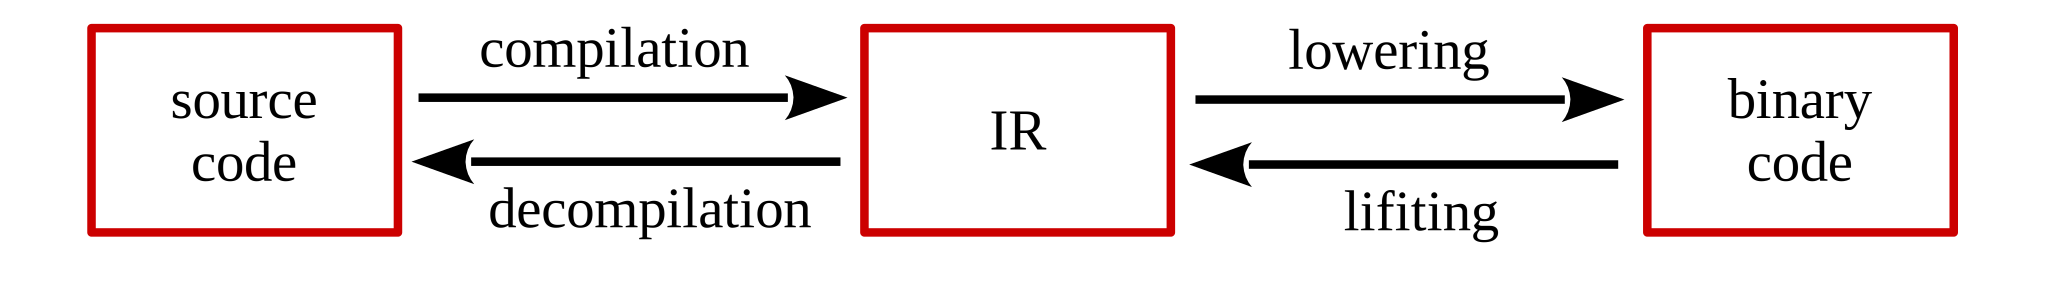
\includegraphics[width=.7\columnwidth]{images/compiler} 
\end{figure}

\vspace{2em}
\mynote{Notes from D\&E start here} For software such as common off-the-shelf programs, neither users nor attackers have access to their source code: 

Challenges (e.g., ~\cite{BITBLAZE-ICISS08}):
\begin{enumerate}
\item Complexity of the instruction sets
\item Lack of a higher-level semantics (functions/CFG, types, buffers)
\item Obfuscation/dynamic code generation
\end{enumerate}

Symbolic techniques may work on the source code or on the binary code. However, it is not uncommon that both the former and the latter work by reasoning on an intermediate representation of the original code. For instance, ~\cite{KLEE-OSDI08} interprets the LLVM bytecode generated by compiling the source code, while~\cite{ANGR-SP16} reasons on the VEX IR that has been obtained by lifting the binary code.


% !TEX root = appendix.tex

\section{Sample Applications}
\label{se:applications}

%\revedit{
The last decade has witnessed an increasing adoption of symbolic execution techniques not only in the software testing domain, but also to address other compelling engineering problems such as automatic generation of exploits or authentication bypass. We now discuss \iffullver{three prominent}{prominent} applications of symbolic execution techniques to these domains. Examples of extensions to other areas can be found, e.g., in~\cite{CGK-ICSE11}.
%}

%The last decade has witnessed an increasing adoption of symbolic execution techniques not only in the software testing domain, but also to address other compelling engineering problems such as automatic generation of exploits or authentication bypass. We now discuss \iffullver{three prominent}{prominent} applications of symbolic execution techniques to these domains. Examples of extensions to other areas can be found, e.g., in~\cite{CGK-ICSE11}.

\subsection{Bug Detection}\mynote{Rendere piu' di ampio respiro il titolo di questa sezione? Keyword: software testing, program understanding}
\label{ss:bug-detection}

Software testing strategies typically attempt to execute a program with the intent of finding bugs. As manual test input generation is an error-prone and usually non-exhaustive process, automated testing technique have drawn a lot of attention over the years. Random testing techniques such as fuzzing are cheap in terms of run-time overhead, but fail to obtain a wide exploration of a program state space. Symbolic and concolic execution techniques on the other hand achieve a more exhaustive exploration, but they become expensive as the length of the execution grows: for this reason, they usually reveal shallow bugs only.

\cite{RK-ICSE07} proposes {\em hybrid concolic testing} for test input generation, which combines random search and concolic execution to achieve both deep program states and wide exploration. The two techniques are interleaved: in particular, when random testing saturates (i.e., it is unable to hit new code coverage points after a number of steps), concolic execution is used to mutate the current program state by performing a bounded depth-first search for an uncovered coverage point. For a fixed time budget, the technique outperforms both random and concolic testing in terms of branch coverage. The intuition behind this approach is that many programs show behaviors where a state can be easily reached through random testing, but then a precise sequence of events -- identifiable by a symbolic engine -- is required to hit a specific coverage point.

% which uses preconstraining on the program states to ensure consistency
\cite{DRILLER-NDSS16} refines this idea and devises a vulnerability excavation tool based on {\sc Angr}~\cite{ANGR-SSP16}, called Driller, that interleaves fuzzing and concolic execution to discover memory corruption vulnerabilities. The authors remark that user inputs can be categorized as {\em general} input, which has a wide range of valid values, and {\em specific} input: a check for particular values of a specific input then splits an application into {\em compartments}. Driller offloads the majority of unique path discovery to a fuzzy engine, and relies on concolic execution to move across compartments. During the fuzzy phase, Driller marks a number of inputs as interesting (for instance, when an input was the first to trigger some state transition) and once it gets stuck in the exploration, it passes the set of such paths to a concolic engine, which preconstraints the program states to ensure consistency with the results of the native execution. On the dataset used for the DARPA Cyber Grand Challenge qualifying event, Driller could identify crashing inputs in 77 applications, including both the 68 and 16 applications for which fuzzing and symbolic execution alone succeeded, respectively. For 6 applications, Driller was the only one to detect a vulnerability.

% temporaneamente messo qui
\mytempedit{
	Maintenance of large and complex applications is a very hard task. Fixing bugs can sometimes even introduce new and unexpected issues in the software, which in turn may require several hours or even weeks to be detected and properly addressed by the developers. \cite{QRL-TOSEM12} tackles the problem of identifying the root cause of failures during regression testing. Given a program $P$ and a newer revision of the program $P'$, if a testing input $t$ generates a failure in $P'$ but not in  $P$, then symbolic execution is used to track the path constraints $\pi$ and $\pi'$ when executing $P$ and $P'$ on the failing input $t$, respectively. Using a SMT solver, a new input $t'$ is generated by solving the constraint $\pi ~\wedge \neg\pi'$. If $t'$ exists (i.e., the constraint is satisfiable), then $P'$ has one or more {\em deviations} in the control-flow graph with respect to $P$ that can be the root cause of the failure. By carefully tracking branch conditions during symbolic execution, \cite{QRL-TOSEM12} are even able to pinpoint which branches are responsible for these deviations. If $\pi \wedge \neg\pi'$ is not satisfiable, then the symmetric constraint query $\neg\pi \wedge \pi'$ is tested and a similar reasoning is performed to detect the possible branch conditions that may have lad to the failure. If $\neg\pi \wedge \pi'$ is also unsatisfiable, then \cite{QRL-TOSEM12} cannot determine the root cause of the problem.

	Another interesting work that targets the problem of software regressions through the use of symbolic execution is~\cite{BOR-ICSE13}. This work introduce an approach called {\em partition-based regression verification} that combines the advantages of both regression verification (RV) and regression testing (RT). Indeed, RV is a very powerful technique for identifying regressions but hardly scales over large programs due to the difficulty in proving behavioral equivalence between the original and the modified program. On the other hand, RT allows to check a modified program for regressions by testing selected concrete sample inputs, making it more scalable but providing limited verification guarantees. The main intuition behind partition-based regression verification is to identify {\em differential partitions}. Each differential partition can be seen as a subset of the input space for which the two program versions -- given the same path constraints -- either expose the same output ({\em equivalence-revealing partition}) or produce different outputs ({\em difference-revealing partition}). For each partition, a test case is generated and added to the regression test suite, which can later be used by a developer for classical RT. Since differential partitions are derived exploiting symbolic execution, this approach suffers from the common limitations that come with this technique. However, if the exploration is interrupted (e.g., due to excessive time or memory usage), partition-based regression verification can still provide guarantees over the subset of input space that has been covered by the detected partitions.

	Static data flow analysis tools can significantly help developers tracks malicious data leaks in software applications. Unfortunately, they often report several allegedly bugs that only after manual inspection can be regarded as false positives. To mitigate this issue,~\cite{ARH-SOAP15} has proposed TASMAN, a system that, after performing data flow analysis to track information leaks, uses symbolic backward execution (SBE) to test each reported bug. Starting from a leaking statement, TASMAN backwards into the code, pruning any path that can be proved to be unfeasible. If all the paths starting from the leaking statement are discarded by TASMAN, then the reported bug can be marked as a false positive.

	Although symbolic execution has been extensively used for bug detection, during the last decades several works~\cite{GDV-ISSTA12,FPV-ICSE13,CLL-ICSE16} have shown how it can be also used for other program understanding activities. For instance,~\cite{GDV-ISSTA12} has introduced {\em probabilistic symbolic execution}, an approach that makes it possible to compute the probability of executing different code portions of a program. This is achieved by exploiting model counting techniques, such as the {\tt LattE}~\cite{LHT-JSC04} toolset, that allows~\cite{GDV-ISSTA12}  to determine the number of solutions for the different path constraints given by the alternative execution paths of a program. The paper by~\cite{FPV-ICSE13} makes a step further and uses probabilistic symbolic execution for performing software reliability analysis. This is computed as the probability of executing any path that has been labeled as successful given a usage profile. Intuitively, a usage profile can be seen as the distribution over the input space. Since in general the termination of symbolic execution cannot be guaranteed in presence of loops, then~\cite{FPV-ICSE13} resorts to bounded exploration. Nonetheless, they define a metric for evaluating the confidence in their reliability estimation, allowing a developer to increase the bounds in order to improve the confidence value. Of a different flavor is the work by~\cite{CLL-ICSE16} that exploits probabilistic symbolic execution to conduct performance analysis. Based on usage profiles and on path execution probabilities, paths are classified into two types: {\em low probability} and {\em high probability}. In a first phase, high-probability paths are explored in a way that maximizes path diversity, generating a first set of test inputs. In the second phase, low-probability paths are analyzed using symbolic execution, generating a second set of test inputs that should expose executions characterized by best-execution times and by worst-execution times. Finally, the program is executed using the test inputs generated during the two phases and running times are measured to generate performance distributions. 

	Another interesting application of symbolic execution is presented by~\cite{PPM-CSF18}. Their technique exploits model counting and symbolic execution for computing quantitative bounds on the amount of information that can be leaked by a program through side-channel attacks. 
	
}
%As it is based on {\sc Angr}, Driller adopts an index-based memory model as in Section~\ref{ss:index-based-memory} where reads can be symbolic and writes are always concretized. % read/write addresses

\subsection{Bug Exploitation}
\label{ss:bug-exploitation}
Bugs are a consequence of the nature of human factors in software development and are everywhere. Those that can be exploited by an attacker should normally be fixed first: systems for automatically and effectively identifying them are thus very valuable.

{\sc AEG}~\cite{AEG-NDSS11} employs preconditioned symbolic execution to analyze a potentially buggy program in source form and look for bugs amenable to stack smashing or return-into-libc exploits~\cite{PB-SSP04}, which are popular control hijack attack techniques. The tool augments path constraints with exploitability constraints and queries a constraint solver, generating a concrete exploit when the constraints are satisfiable. The authors devise the {\em buggy-path-first} and {\em loop-exhaustion} strategies (Table~\ref{tab:heuristics}) to prioritize paths in the search. On a suite of 14 Linux applications, {\sc AEG} discovered 16 vulnerabilities, 2 of which were previously unknown, and constructed control hijack exploits for them.

{\sc Mayhem}~\cite{MAYHEM-SP12} takes another step forward by presenting the first system for binary programs that is able identify end-to-end exploitable bugs. It adopts a hybrid execution model based on checkpoints and two components: a concrete executor that injects taint-analysis instrumentation in the code and a symbolic executor that takes over when a tainted branch or jump instruction is met. Exploitability constraints for symbolic instruction pointers and format strings are generated, targeting a wide range of exploits, e.g., SEH-based and jump-to-register ones. Three path selection heuristics help prioritizing paths that are most likely to contain vulnerabilities (e.g., those containing symbolic memory accesses or instruction pointers). A virtualization layer intercepts and emulates all the system calls to the host OS, while preconditioned symbolic execution can be used to reduce the size of the search space. Also, restricting symbolic execution to tainted basic blocks only gives very good speedups in this setting, as in the reported experiments more than $95\%$ of the processed instructions were not tainted. {\sc Mayhem} was able to find exploitable vulnerabilities in the 29 Linux and Windows applications considered in the evaluation, 2 of which were previously undocumented. Although the goal in {\sc Mayhem} is to reveal exploitable bugs, the generated simple exploits can be likely transformed in an automated fashion to work in the presence of classical OS defenses such as data execution prevention and address space layout randomization~\cite{Q-SEC11}. 

\vspace{-1mm} % TODO
\subsection{Authentication Bypass}
\label{ss:auth-bypass}
Software backdoors are a method of bypassing authentication in an algorithm, a software product, or even in a full computer system. Although sometimes these software flaws are injected by external attackers using subtle tricks such as compiler tampering~\cite{KRS-TR74}, there are reported cases of backdoors that have been surreptitiously installed by the hardware and/or software manufacturers~\cite{CZF-USEC14}, or even by governments~\cite{NSA-BACKDOOR}. 

Different works~\cite{DMR-USEC13,ZBF-NDSS14,FIRMALICE-NDSS15} have exploited symbolic execution for analyzing the behavior of binary firmwares. Indeed, an advantage of this technique is that it can be used even in environments, such as embedded systems, where the documentation and the source code that are publicly released by the manufacturer are typically very limited or none at all. For instance,~\cite{FIRMALICE-NDSS15} proposes Firmalice, a binary analysis framework based on {\sc Angr}~\cite{ANGR-SSP16} that can be effectively used for identifying authentication bypass flaws inside firmwares running on devices such as routers and printers. Given a user-provided description of a privileged operation in the device, Firmalice identifies a set of program points that, if executed, forces the privileged operation to be performed. The program slice that involves the privileged program points is then symbolically analyzed using {\sc Angr}. If any such point can be reached by the engine, a set of concrete inputs is generated using an SMT solver. These values can be then used to effectively bypass authentication inside the device. On three commercially available devices, Firmalice could detect vulnerabilities in two of them, and determine that a backdoor in the third firmware is not remotely exploitable.
% !TEX root = paper.tex
\section{Conclusions}
\label{se:conclusions}

Techniques for symbolic execution have evolved significantly in the last decade, leading to major practical breakthroughs. In 2016, the DARPA Cyber Grand Challenge hosted systems that can detect and fix vulnerabilities in unknown software with no human intervention, such as {\sc Angr}~\cite{ANGR-SSP16} and {\sc Mayhem}~\cite{MAYHEM-SP12}, which won the \$2M first prize. {\sc Mayhem} was also the first autonomous software to play the Capture-The-Flag contest at the DEF CON 24 hacker convention. The event demonstrated that tools for automatic exploit detection based on symbolic execution can be competitive with human experts, paving the road to unprecedented applications and the rise of start-ups that have the potential to shape software security and reliability in the next decades. 

For details on the techniques behind symbolic executors, we would like to suggest the interested reader to have a look at a survey we have recently completed. The survey, available at \url{https://arxiv.org/abs/1610.00502}, has been written with the goal of providing an overview of the main ideas, challenges, and solutions developed in the area, distilling them for a broad audience.

\iffalse

Techniques for symbolic execution have evolved significantly in the last decade, leading to major practical breakthroughs. In 2016, the DARPA Cyber Grand Challenge hosted systems that can detect and fix vulnerabilities in unknown software with no human intervention, such as {\sc Angr}~\cite{ANGR-SSP16} and {\sc Mayhem}~\cite{MAYHEM-SP12}, which won the \$2M first prize. {\sc Mayhem} was also the first autonomous software to play the Capture-The-Flag contest at the DEF CON 24 hacker convention\footnote{\url{https://www.defcon.org/html/defcon-24/dc-24-ctf.html}.}. The event demonstrated that tools for automatic exploit detection based on symbolic execution can be competitive with human experts, paving the road to unprecedented applications %and the rise of start-ups 
that have the potential to shape software %security and 
reliability in the next decades. 

This survey has discussed some of the key aspects and challenges of symbolic execution, presenting them for a broad audience. To explain the basic design principles of symbolic executors and the main optimization techniques, we have focused on single-threaded applications with integer arithmetic. Symbolic execution of multi-threaded programs is treated, e.g., \iffullver{in~\cite{KPV-TACAS03,SA-HVC06,CLOUD9-EUROSYS11,FHR-ESEC13,BGC-OOPSLA14,GKW-ESEC15}}{in~\cite{FHR-ESEC13,BGC-OOPSLA14,GKW-ESEC15}}, while techniques for programs that manipulate floating point data are addressed \iffullver{in, e.g., \cite{M-STVR01,BGM-STVR06,LTH-ICTSS10,CCK-EUROSYS11,BVL-POPL13,CCK-TSE14,RPW-SIGSOFT15}}{in, e.g., \cite{BVL-POPL13,CCK-TSE14,RPW-SIGSOFT15}}.

We hope that this survey will help non-experts grasp the key inventions in the exciting line of research of symbolic execution, inspiring further work and new ideas.

\ifdefined\arxivver

\myparagraph{Acknowledgements}
This work is supported in part by a grant of the Italian Presidency of the Council of Ministers and by the CINI (Consorzio Interuniversitario Nazionale Informatica) National Laboratory of Cyber Security.

\myparagraph{Live Version of this Article}
We complement the traditional scholarly publication model by maintaining a live version of this article at {\href{https://github.com/season-lab/survey-symbolic-execution}{https://github.com/season-lab/survey-symbolic-execution/}}. The live version incorporates continuous feedback by the community, providing post-publication fixes, improvements, and extensions.
\fi

\fi

%------------------------------------------------------------------------------

\iffalse
\section{Misc}
\label{se:misc}

The references list is condensed. The default bibliography styles, such as \texttt{plain}, \texttt{abbrv}, and \texttt{alpha}, are suggested.

Page numbers are at the bottom of every page. Authors must leave the page numbers in as-is. When EasyChair proceedings and Procedia volumes are processed by EasyChair, the correct volume page numbers will be inserted automatically.

Paragraph headings should not be capitalized and should have a trailing period. 

References must be provided in a {\tt .bib} file, so that \BibTeX\ can be used to generate the references in a consistent style in a volume. The preferred styles are {\tt plain} and {\tt alpha}.
\fi

\bibliographystyle{plain}
%\bibliographystyle{alpha}
%\bibliographystyle{unsrt}
%\bibliographystyle{abbrv}
\bibliography{symbolic}

%------------------------------------------------------------------------------
\appendix
\section{Appendix}
\label{se:appendix}

\noindent Depending on the specific context in which symbolic execution is used, different choices and assumptions are made to address the questions highlighted above. Although these choices typically affect soundness or completeness, in several scenarios a partial exploration of the space of possible execution states may be sufficient to achieve the goal (e.g., identifying a crashing input for an application) within a limited time budget.

%------------------------------------------------------------------------------
% Index
%\printindex

%------------------------------------------------------------------------------
\end{document}

